\documentclass[a4paper]{report}
\usepackage[T1]{fontenc}
\usepackage[utf8]{inputenc}
\usepackage[english]{babel}
\usepackage{titlesec}
\usepackage{lipsum}
\usepackage{booktabs}
\usepackage{hyperref}
\usepackage{graphicx}
\usepackage{float}
\usepackage{rotating}
\usepackage[dvipsnames]{xcolor}
\usepackage{listings}
\usepackage[shortlabels]{enumitem}
\usepackage{geometry}
\usepackage{pdflscape}
\usepackage{caption}
\usepackage{soul}
\usepackage{blindtext}
\usepackage{array}
\graphicspath{{./images/}}
\begin{document}

%%The two following lines remove the line "Chapter n" at the beginning of each chapter, before the title
%\titleformat{\chapter}[display]
%  {\normalfont\bfseries}{}{0pt}{\Large}
\titleformat{\chapter}[hang] 
{\normalfont\huge\bfseries}{\thechapter}{1em}{} 

\title{CPMS system design}
\author{Federico Bono, Daniele Cipollone}
\date{\today}

\newcommand\descitem[1]{\item{\bfseries #1}\\}

\begin{titlepage}
\begin{figure}[t]
\centering
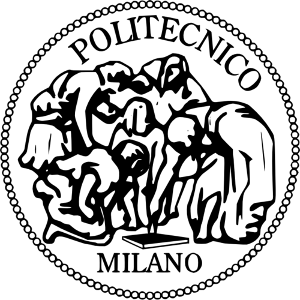
\includegraphics[width=0.3\textwidth]{Logo}
\end{figure}
\begin{center}
    \textsc{ \LARGE{Politecnico di Milano \\}}
	\textsc{ \Large {School of Industrial and Information Engineering\\ }}
	\textnormal{ \Large{Master of Science in Computer Science and Engineering\\}}
	\vspace{3mm}
	\textnormal{ \Large{Software Engineering 2 Project\\}}
	\vspace{30mm}
	\fontsize{10mm}{7mm}\selectfont 
    \textup{eMall - eMSP system}\\
    \textnormal{ \LARGE{Requirement Analysis and Specification Document\\}}
\end{center}

\vspace{18mm}

\begin{center}
    \textnormal{\large{\bf Authors:\\}}
	{\large Federico Bono \\ Daniele Cipollone}
	\fontsize{10mm}{5mm}\selectfont 
\end{center}
\vspace{15mm}

\centering{\large{
Academic Year 2022/2023 \\
\vspace{10mm}
Milano, 06/01/2023 \\
\vspace{2mm}
Version 1.2
}}

\end{titlepage}


\newgeometry{top=3cm}
\tableofcontents
\listoffigures
\restoregeometry

\chapter{Introduction}
\section{Purpose}
The purpose of this document is to describe and explain in details the design choices for the development and deployment of the eMSP system of eMall. The description is structured on multiple levels to give an overview of the system from multiple viewpoints. In the following pages you will find:

\begin{enumerate}
	\item High level overview of the architecture
	\item Overview of the components of the system
	\item Deployment overview
	\item Overview of the interactions between components
	\item Overview of the interfaces offered by the various components
	\item The UI of the mobile application used by the final user
	\item The patterns and technologies used in the system
\end{enumerate}

\section{Scope}
eMall App is a platform that helps the end users to plan the charging process, by getting information about Charging Points nearby, their costs and any special offer; book a charge in a specific point, control the charging process and get notified when the charge is completed. It also handles payments for the service.\\\\
In the e-Charging ecosystem, there are many different actors involved that we need to keep into consideration while collecting requirements and designing the system. The first information to consider is that Charging Points are owned and managed by Charging Point Operators (CPOs) and each CPO has its own IT infrastructure, managed via a Charge Point Management System (CPMS). \\\\
In order to comunicate with the various CPMS, the 
\href{../Specs/OCPI-2.2.1.pdf}{OCPI (Open Charge Point Interface) protocol} is used.\\\\
To be able to process payments, the system will need to communicate with a Payment Service Provider (PSP) via the HTTP(s) protocol, using the propertary APIs offered by the provider.\\\\
Given that our system is not the producer of the data, and that there is the need for implementing different functionalities (e.g. payments) a three-tier architecture has been chosen, to separate the data layer (that mostly acts as a cache layer) and the business logic layer.


\section{Definitions, Acronyms, Abbreviations}

\subsection{Definitions}
\begin{tabular}{|p{5cm}|p{10cm}|}
	\hline
	Connector \newline Charging Socket & Physical connector that allow to transfer energy to the connected vehicle\\
	\hline
	Charging slot & Physical device with multiple Connectors that can charge electric vehicles.\newline
	NOTE: from OCPI definitions a Charging Slot can have up to one connector active at any time (i.e. can charge only one Vehicle at any time) \\
	\hline
	Charging Point & Physical structure composed by multiple Charging Slots\\
	\hline
	Maintenance of a charging slot & Activity/activities that results in a momentary unavailability of the charging slot\\
	\hline
	Payment information & information required by the payment provider to be able to charge the user for the service (e.g. credit card number)\\
	\hline
	Charging session & period of time when the vehicle is connected to a charging plug for charging\\
	\hline
	Booking period & period of time between the booking of a charging session and the beginning of the charging session\\
	\hline
	{Guest \newline Guest User} & Unregistered user\\
	\hline
	{User \newline Enabled User \newline Active User} & Registered user with confirmed email and payment method\\
	\hline
	Unconfirmed User & Registered user without confirmed email\\
	\hline
	Pending User & Registered user with confirmed email but no payment method set up\\
	\hline
	Payment Service Provider & External service that provides API to process payments\\
	\hline
\end{tabular}

\subsection{Acronyms}
\begin{tabular}{|l|l|}
	\hline
	eMSP & e-Mobility Service Provider\\
	\hline
	CP & Charge Point / Charging Point\\
	\hline
	CPO & Charging Point Operator\\
	\hline
	CPMS & Charging Point Management System\\
	\hline
	OCPI & Open Charge Point Interface\\
	\hline
	EV & Electric Vehicle\\
	\hline
	PSP & Payment Service Provider\\
	\hline
	API & Application Programming Interface\\
	\hline
\end{tabular}


\section{Revision History}
\begin{itemize}
	\item v1.0 - 05 January 2023
\end{itemize}

\section{Related Documents}
\begin{itemize}
	\item {eMSP RASD (RASD\_eMSP.pdf)}
	\item OCPI specifications document (OCPI-2.2.1.pdf)
\end{itemize}

\section{Document structure}
The document is structured in six sections:

\begin{enumerate}
	\item Description and introduction of the various design choices made during the design of the system. Descriptions are written at different levels of abstractions: from the general point of view to the detailed view of the single component.
	\item User interfaces and design mockups.
	\item The requirement traceability matrix is used to map each component to the requirement(s) that fulfils.
	\item Implementation and test plans for the entire system
	\item Total effort
	\item References used
\end{enumerate}























\chapter{Architectural Design}
\section{Overview: high-level components and interactions}

As anticipated in the previous chapter, the architecture selected for the design and development of the system is the three-tier architecture.

This architecture allow us to split the implementation into three layers:
\begin{enumerate}
	\item Presentation: is the mobile application that will be used by the final users. It allows all the interactions with the system and will also be used as a communication endpoint for the notifications.
	\item Application: is the backend of the system, all the business logic and the various connections between the system and the external services are implemented here.
	\item Data: is the layer responsible to expose connectivity interfaces from the database. It will be a DBMS.
\end{enumerate}
All the layers communicate in a linear way: the Presentation one interacts only with the Application layer, the same as the Data layer. With this architecture the presentation and the Data layers have no direct communication path, this allow to develop all the business logic only in the Application layer.
Other advantages of using this architecture are that the various layers can be developed with different technologies and that they can be duplicated and differentiated (i.e. there can be multiple presentation layers that interact with the same application layer)

The main reasons behind the choice are:
\begin{itemize}
	\item We are not the producer of the data
	\item We need to integrate different external services
	\item Separate the business logic from the data to:
	\begin{itemize}
		\item Allow a parallel development with multiple teams specialized in the single tiers
		\item Allow to use different technologies for the different tiers
	\end{itemize}
\end{itemize}


\begin{figure}[h]
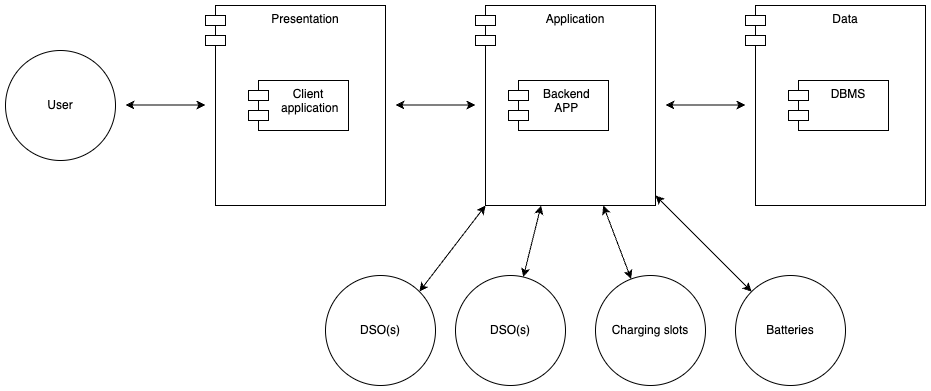
\includegraphics[width=\textwidth]{component_diagrams/overview}
\caption{Overview of the chosen three-tier architecture with actors}
\end{figure}

\clearpage

\section{Component view}
The following schema shows all the main components and interfaces of the system. Later on you will find the details of each component.


\begin{figure}[h]
\centering
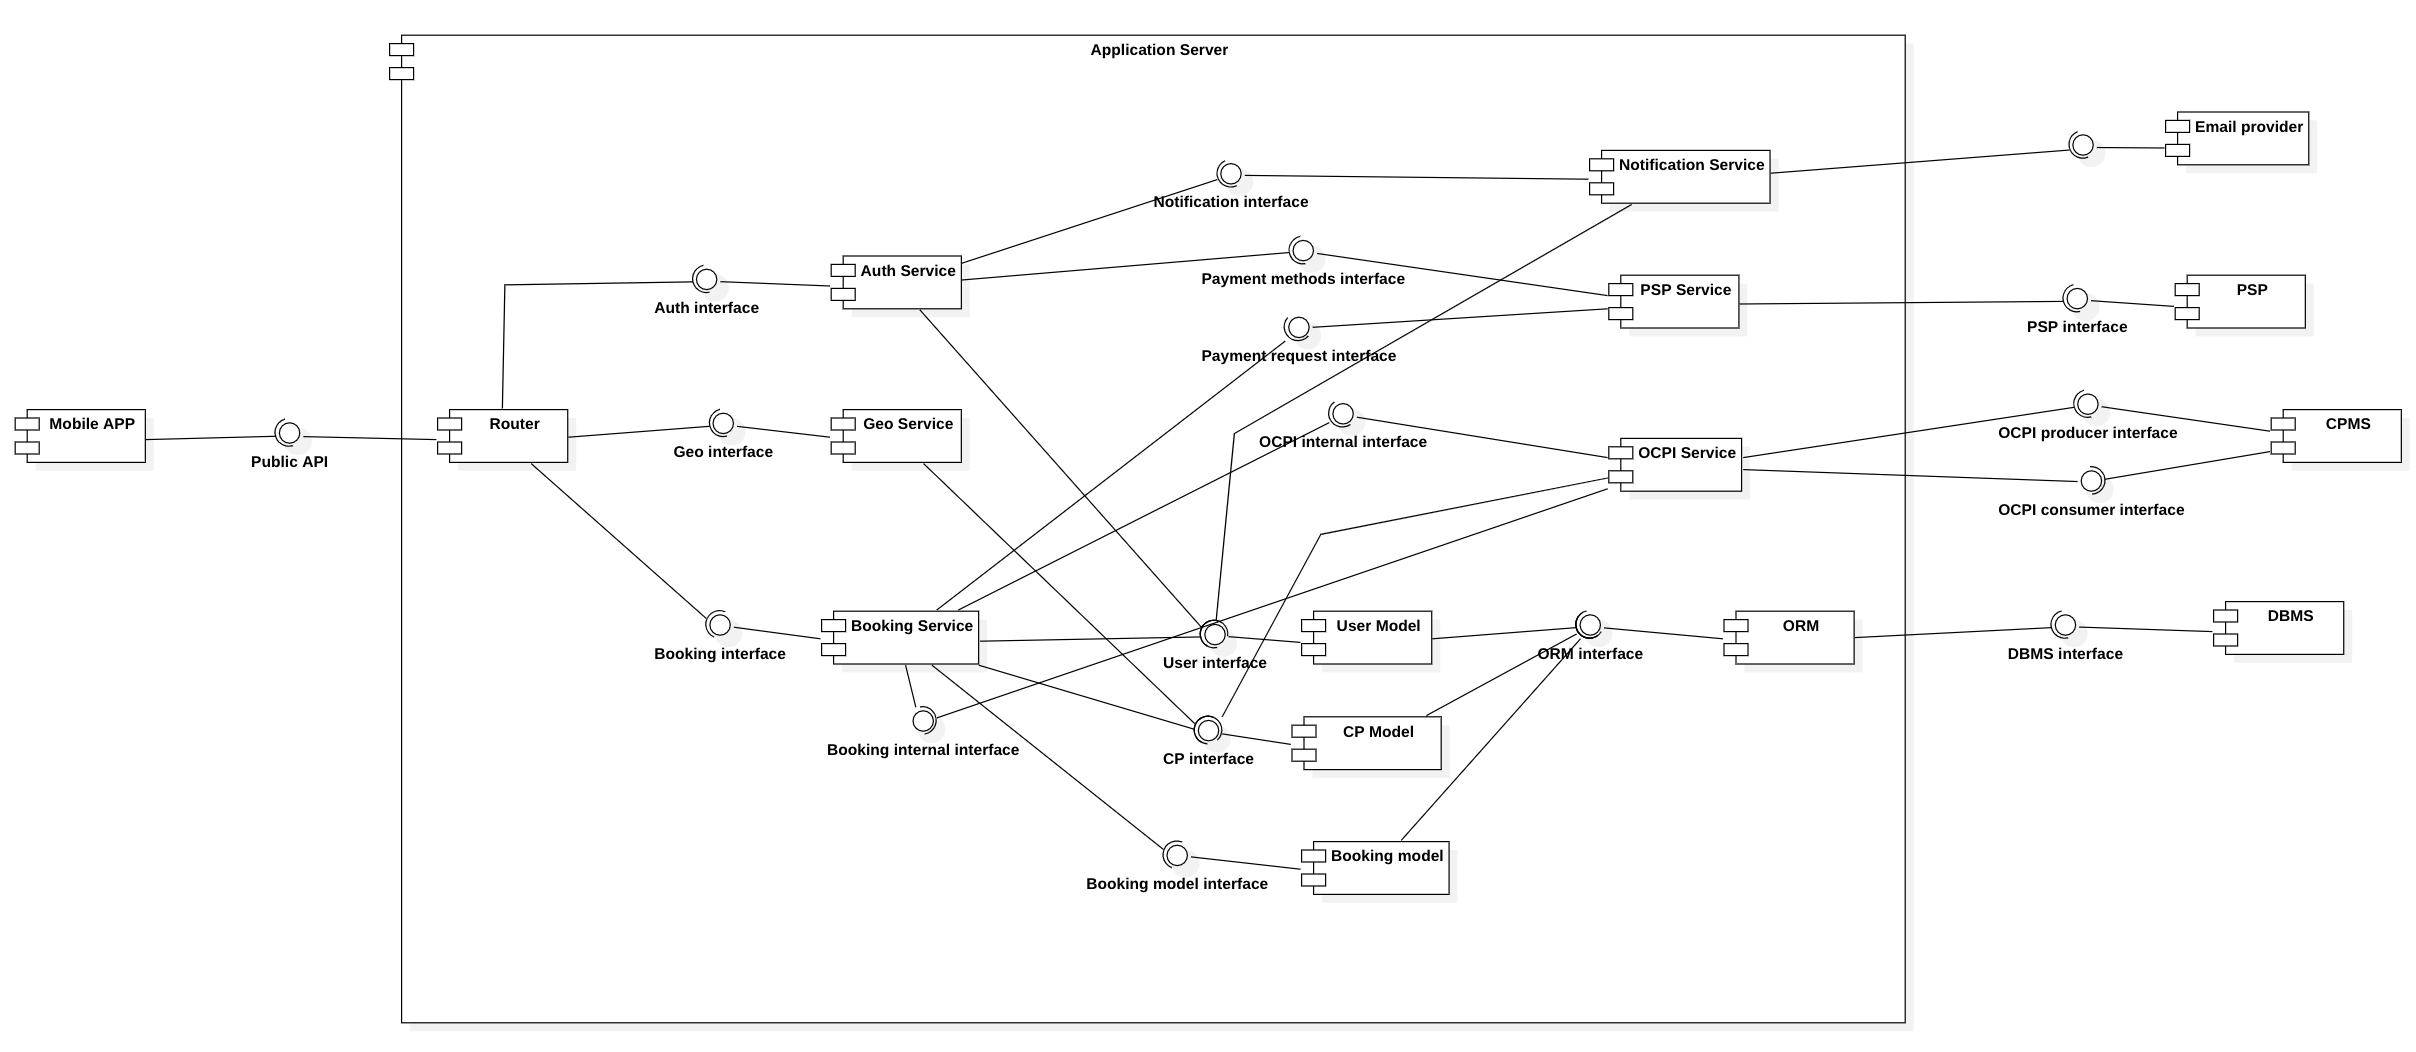
\includegraphics[angle=90,origin=c,height=14cm]{component_diagrams/component_diagram}
\caption{Component diagram of the system}
\end{figure}

\clearpage
\newpage

\begin{itemize}
	\item Application server: not a real "component" it shows the division between the backend, the frontend, the data layer and the external service. In the three-tier architecture it represents the Application layer.
	\item Mobile APP: mobile application for the system, used by the users.
	\item Router: handles all the requests directed to the Application APIs (i.e. OCPI PUSH endpoints are not handled here) that comes into the Application Server, uses the Auth Service to Authenticate and Authorize them. After that, if all the checks are passed, it will forward the request to the correct service that exposes the required route. It basically acts as a middleware, its presence is useful as it acts as a single point to develop all the authentication/authorization logic so that if it needs changes we can just update the router (and eventually the auth service) instead of updating all the services.
	\item Auth Service: is an internal service that handles authentication (Signup and login) and authorization (even if at the moment our system does not need that). It is mainly used internally but it exposes a couple of endpoints to the router for both signup and login.
	\item Geo Service: an highly reusable service, it uses a set of geographical points and exposes functionalities to list, filter and search those points based on their position. For our system is needed for the map functionality of the Mobile APP.
	\item Booking Service: it manages the booking for the application, it exposes some endpoints to the router for the booking functionalities of the Mobile APP and it is also used from other internal services.
	\item Notification Service: it manages all the notifications that the system needs to send to the user, both via email as via push services (e.g. Firebase Cloud Messaging)
	\item PSP Service: it manages the communication with the Payment Service Providers, it is useful as we can easily swap it with proprietary SDKs from the various providers.
	\item OCPI Service: it manages the communication with the CPMS, it exposes the endpoints for the PUSH part of the protocol (is needed to receive real-time updated from CPMS)
	\item ORM: a library that allows an easy to use mapping between Models and DB table, it handles queries and relationships. It is not worth it to develop an in-house solution, so we will use a library for that.
	\item User Model, CP Model, Booking Model: Models components that sit between services and ORM, useful to attach event listeners and other effects that need to run when updating the data. 
	\item Email Provider: external service (or services) that exposes API to send emails
	\item PSP: external service that exposes API to process payment
	\item CPMS: Charging Point Management System that exposes OCPI compliant API
	\item DBMS: Database Management System
\end{itemize}





















\chapter{User Interface}


\subsection{Search for a Charge Point}
\begin{figure}[h]
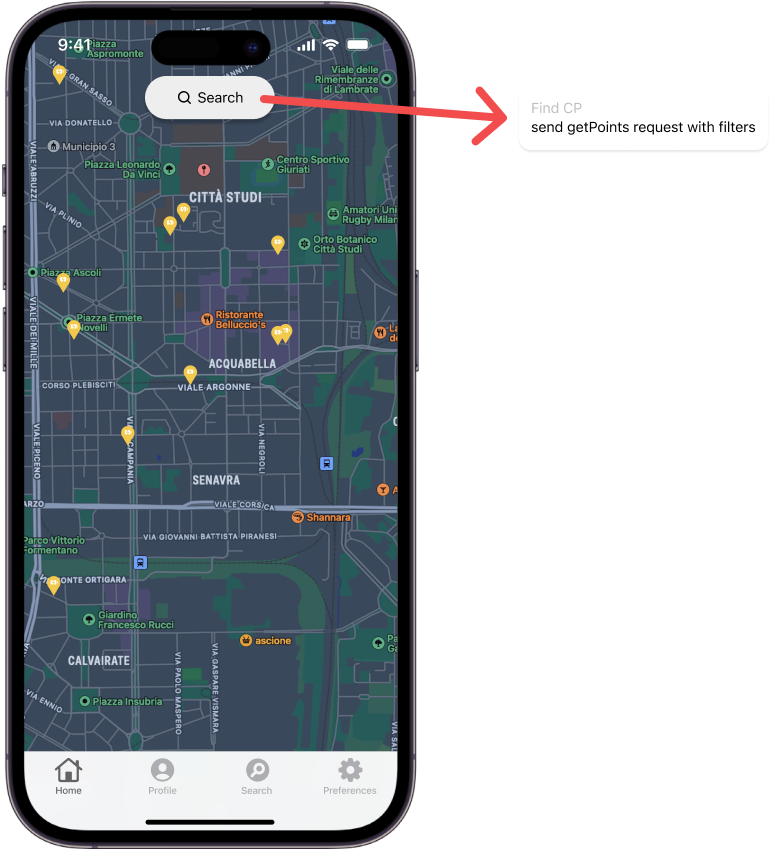
\includegraphics[width=10cm]{UI/search}
\caption{Search for a Charge Point}
\end{figure}
In this first view, the user has the ability to view all the CP nearby via the map. The datapoints are loaded via an API request to the Geo Service that returns all the points. The user can also search for a specific CP using both the "Search" button on the upper part of the map, as also using the tab button on the bottom of the application.


\subsection{Details of a CP and booking of a session}
\begin{figure}[h]
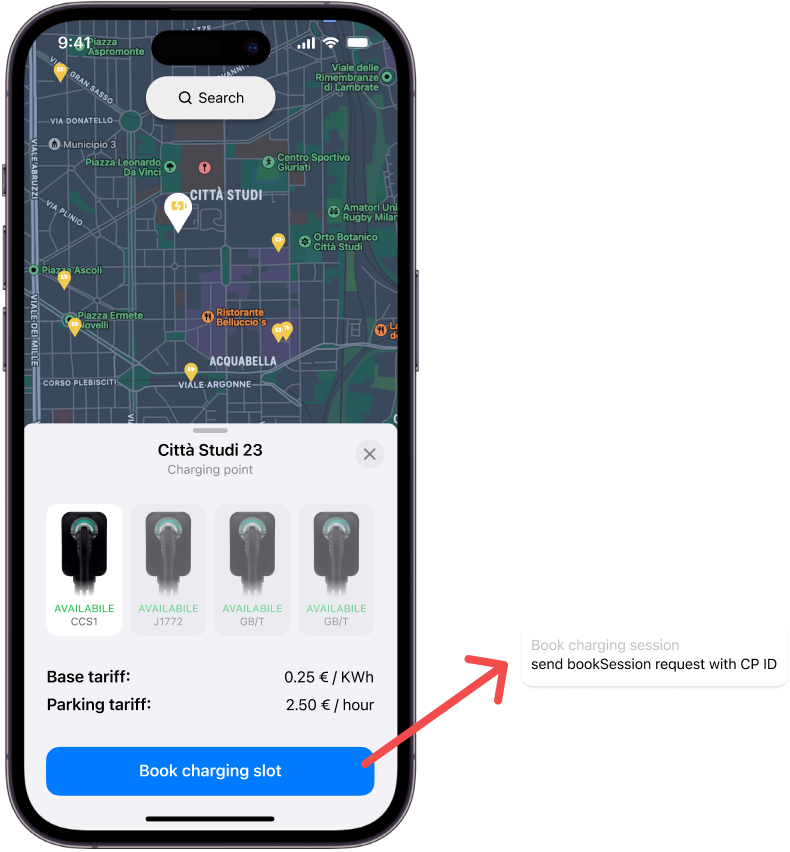
\includegraphics[width=10cm]{UI/booking}
\caption{Details of a CP and booking of a session}
\end{figure}
After tapping on a CP icon on the map, the user will be presented with the details of the selected CP, with all the plugs available and the tariffs.
Then, the user can decide to book the charging slot by selecting the connector type that he needs and by tapping onto the "Book charging slot" button. 
A bookSession request is forwarded to the Booking Service, than the OCPI Service is used to send the correct request to the selected CPMS.
After some time the CPMS will push the session to the eMSP system and the Notification Service will send a push notification to the user and will update the UI
\clearpage


\subsection{Starting the charging process}
\begin{figure}[h]
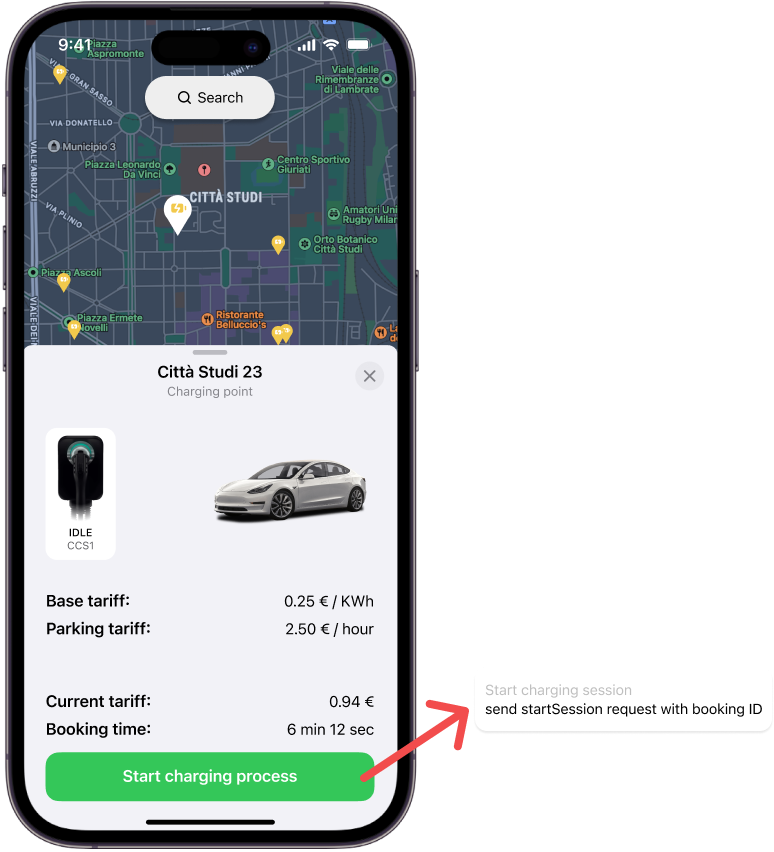
\includegraphics[width=10cm]{UI/start}
\caption{Starting the charging process}
\end{figure}
After the update received by the CPMS, a session will start and the booking details will be updated to show the current tariff that will be applied and the booking time already passed. The user, once he's reached the CP and has connected the EV to the station, can start the charging process via the "Start charging process" button. The startSession request will be sent to the Booking Service that will forward the request to the CPMS by using the OCPI Service. As the previous request, the CPMP will push the update on the booking session.
\clearpage

\subsection{Completing the charging process}
\begin{figure}[h]
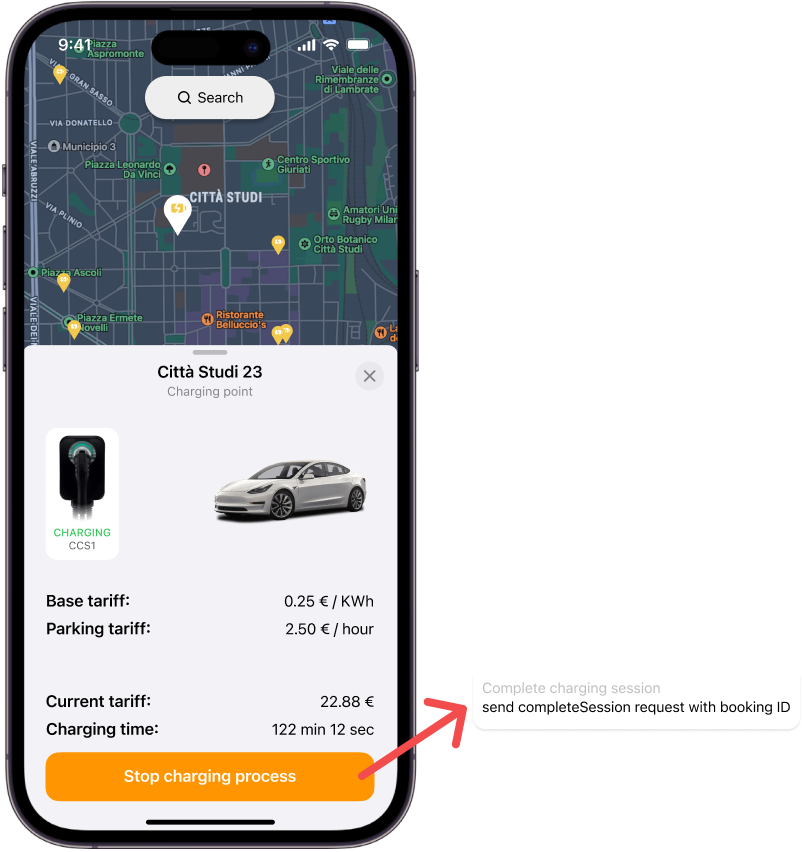
\includegraphics[width=10cm]{UI/complete}
\caption{Completing the charging process}
\end{figure}

At any time the user can view the status of the booking, updated with the latest info pushed by the CPMS. He can also complete the charging process by tapping the "Stop charging process" button. A completeSession request will be forwarded via the Booking Service to the OCPI Service that will send the correct command to the CPMS. After the confirmation from the CPMS, the user will be charged automatically via the PSP Service with the complete tariff communicated by the CPMS.
\clearpage

\subsection{Push notification from Charging Point}
\begin{figure}[h]
\centering
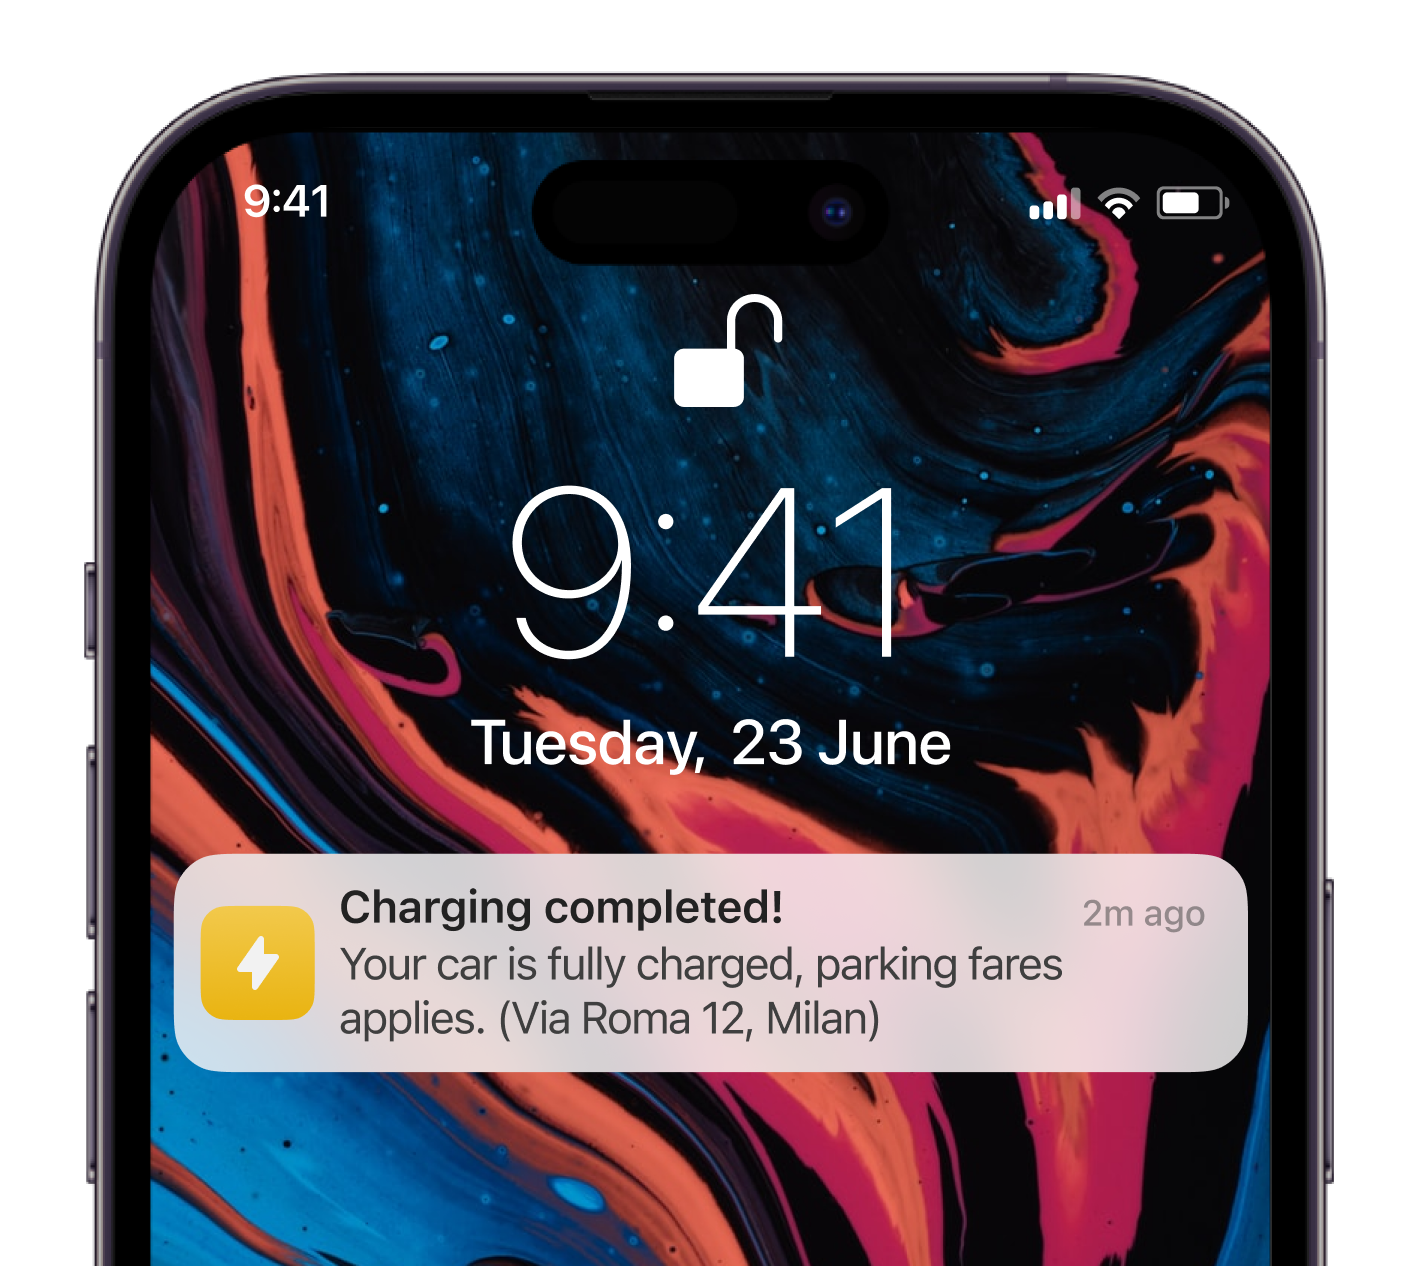
\includegraphics[width=10cm]{UI/notification}
\caption{Push notification from Charging Point when the charging session has been completed}
\end{figure}

When the CPMS push an update to the system to notify the end of the charging process, the System will send a push notification to the user, reminding them that the parking fares might be applied.










\chapter{Requirements Traceability}
\section{Functional requirements}
In the following table are summarized the requirements extracted from the RASD.\\

\begin{tabular}{|c|l|}
	\hline
	\bf{Requirement} & \bf{Description} \\
	\hline
	R1 & Allow to book a charging session on a specific CS\\
	\hline
	R2 & Allow to start a charging session on a specific CS\\
	\hline
	R3 & Allow to stop a charging session on a specific CS\\
	\hline
	R4 & Forward information about the state of a charging session to the eMSP\\
	\hline
	R5 & Allow Login for CPO\\
	\hline
	R6 & Allow to view information about the internal status of a charging station\\
	\hline
	R7 & Forward of the offered tariffs\\
	\hline
	R8 & Allow CPO to set or change tariffs\\
	\hline
	R9 & Allow CPO to enter static information about charging stations\\
	\hline
	R10 & Forward information about the location of charging stations\\
	\hline
	R11 & Forward information about the location of charging stations\\
	\hline
	R12 & Allow CPOs to change the settings and management settings of the charging station\\
	\hline
\end{tabular}
\pagebreak
\section{Components mapping}
To keep the mapping simple, we define some abbreviations for the components.\\

\begin{tabular}{|c|l|}
	\hline
	\bf{} & \bf{Component} \\
	\hline
	AS & Application Server\\
	\hline
	ESS & External Status Service\\
	\hline
	BS & Booking Service\\
	\hline
	APP & Client Application\\
	\hline
	RT & Router\\
	\hline
	AT & Auth Service\\
	\hline
	ISS & Internal Status Service\\
	\hline
	DPS & Dynamic Pricing Service\\
	\hline
	EMS & Energy Management Service\\
	\hline
	DSOS & DSO service\\
	\hline
	OCPPS & OCPP Service\\
	\hline
	BMS & Battery Manager Service\\
	\hline
	OC & OCPI Service\\
	\hline
	OR & ORM\\
	\hline
	MD & Models (User, CP, Booking Model...)\\
	\hline
\end{tabular}

\section{Components mapping on Requirements}

\begin{tabular}{|p{1.5cm}|p{3cm}|p{10cm}|}
	\hline
	\bf{Comp.} & \bf{Requirements} & \bf{Reason} \\
	\hline
	\hline
	AS & R* & Application server is needed for all the functionalities as it is the foundation for the system\\
	\hline
	ESS & R4, R7,R11 &  External Status Service is used to send and analyze data regarding the external state of the system\\
	\hline
	BS & R1-3 & Booking Service manages the "state machine" and the related effects for the charging sessions.\\
	\hline
	APP & R5-6,R8-9,R12 & Client Application is the medium for the communication between the CPO and the system \\
	\hline
	RT & R5-6,R8-9,R12 & Router is the middleware component for the "frontend" functionalities.\\
	\hline
	AT & R5-6,R8-9,R12 & Authentication Service allows to check the state of the user\\
	\hline
	ISS & R6 & Internal Status Service is the service that allows to show and analyze data regarding the internal state of the system\\
	\hline
	DPS & R1,R7-8,R11 &Dynamic Pricing Service is the service capable of calculating and indicating active tariffs, which can be dynamic according to electricity prices\\
	\hline
	EMS & R2-3,R9,R12 & Energy Management Service is the component that allows you to manage energy management policies at the various charging stations\\
	\hline
	DSOS & R8,R13 & It allows the bidirectional communication with the various DSOs\\
	\hline
	OCPPS & R2-4,R6,R9-10  & It allows the bidirectional communication with the various CS/EVSE\\
	\hline
	BMS &  R9,R12-13 & Battery Manager Service allows communication with the various batteries and their administration\\
	\hline
	OC & R1-R4,R7,R10 & It allows the bidirectional communication with the various eMSP\\
	\hline
	OR &  R*& It allows to easily access the DBMS APIs and to manage the relationships between the models\\
	\hline
	MD & R* & It allows to access the ORM interfaces and to trigger functions on models’ events (e.g. send a notification when charging is completed)\\
	\hline
\end{tabular}






















\chapter{Implementation, Integration and test Plan}
\section{Plan details}
To implement the system components we've decided to follow a planned structure, dividing the components into various groups in order to be able to develop them in parallel, using a more complex workforce. Given the limited number of functionalities, we think that a progressive release strategy (i.e. with multiple smaller releases) is not really worth for the final user, that means that the only way to bring value to the user will be to have the system released all at once.\\
This assumption allows us to follow different strategies, both bottom-up and top-down. \\
To keep aligned the tests set and the actual codebase, we decided to follow the famous TDD (Test Driven Development) strategy, where unit/integration tests are written before the code and then the actual codebase is developed to fulfil those tests. \\
To develop the best user experience possible, we decided to follow the top-down approach, splitting the development of the various components by functionalities viewed from the user's point of view. We've can use the goals defined in the RASD as a starting point.\\\\
We've defined the following functionalities:
\begin{enumerate}
	\item Signup, Login, Email confirmation and payment method registration
	\item View the CP locations, filter them and view the details of a location
	\item Book a charge session at a specific location for a specific connector
	\item Start and complete a charge session from the app for a specific booked session
	\item View the list and the details of the booked sessions
	\item Be notified when the charging process has been completed
	\item Be charged with the correct amount after the charging process\\
\end{enumerate}

Based on those functionalities we can define the following development path:
\begin{enumerate}
	\item \textbf{Application scaffolding}\\
	In this phase we set up the servers (from a logical point of view, through docker), the frameworks and the connections with the DBMS. We use the Router component given by the framework, so it can be considered as being developed/integrated in this phase.
	\item \textbf{Authentication and notification scaffolding}\\ In this phase we develop the Authentication Service, the Notification Service and we connect with the chosen Email Provider to send the email confirmation link to the user. The related UI and Models are also developed in this phase, alongside with the needed database migrations.
	\item \textbf{Payment method verification}\\ As we delegate the verification to the PSP, we only need to develop the PSP Service on the backend (with the related models, tables and DB migrations) and integrate the UI on the mobile APP.
	\item \textbf{OCPI service integration}\\ We use some open source libraries that implements the needed interface for the OCPI (both PULL and PUSH methods), and wrap it with a utility service (i.e. the OCPI Service) to expose the chosen interfaces. As we are following the top-down approach we only set up the libraries and the base service.
	\item \textbf{CP list and details}\\ We start to develop the needed interfaces for the OCPI service and then we can start implementing the Geo Service to allow the user to view all the needed information.
	\item \textbf{Booking Service}\\ In this phase we start to develop the functionalities to book a charge from a specific CP, we need to expose those functionalities from the OCPI Service and then we can implement the needed models alongside with the Booking Service and the Mobile APP UI.
	\item \textbf{Charging functionalities}\\ In this phase we add the charging management functionalities to both OCPI Service and Booking Service.
	\item \textbf{Booking status and list}\\ In this phase we use the PUSH interfaces of the OCPI libraries to update our booking model data. We also add the needed functionalities to the Booking Service that will allow the user to view the bookings status.
	\item \textbf{Notifications}\\ We implement a event callback on the Booking Model that will trigger the Notification Service to send a "charging completed" notification to the user devices.
	\item \textbf{PSP integration}\\ We implement another event callback on the Booking Model to trigger the payment from the PSP Service to charge the user for the service.
\end{enumerate}
\newpage

\section{Additional testing}
After development and integration we will run some system-level tests.
First test to run is on non-functional requirements, developers need to test accessibility features and base performance, doing so we can easily find the most important bottlenecks of the application.
Another test that is useful to run is the so called "chaos test": various components of the system are disconnected on purpose to try to verify the behaviour of the system, the goal here is to check that the system fails safely, without losing or leaking data. 
The final test that will be run is the acceptance test: the system will be tested with real users in the production environment to verify that is really useful to them.







\chapter{Effort spent}
\begin{tabular}{|l|l|}
	\hline
	Task & Time spent\\
	\hline
	Introduction & 2 h\\
	\hline
	Architectural Design & 22 h\\
	\hline
	User interface & 5 h\\
	\hline
	Requirements Traceability & 3 h\\
	\hline
	Implementation, Integration and Test Plan & 4 h\\
	\hline
	Revision & 2 h\\
	\hline
\end{tabular}
\chapter{References}

\begin{itemize}
	\item \textbf{TDD (Test Driven Development)} - \url{https://it.wikipedia.org/wiki/Test_driven_development}
	\item \textbf{Three-Tier Architecture} - \url{https://www.ibm.com/topics/three-tier-architecture}
	\item \textbf{OCPI specs} - \url{https://evroaming.org/app/uploads/2020/06/OCPI-2.2-d2.pdf}
	\item \textbf{Chaos Testing} - \url{https://www.ibm.com/garage/method/practices/manage/practice_chaotic_testing/}
	\item \textbf{Acceptance Testing} - \url{https://en.wikipedia.org/wiki/Acceptance_testing#User_acceptance_testing}
\end{itemize}


\end{document}